\part{Getting Started}

\section{Getting Started}
\begin{frame}
	\tableofcontents[currentsection,hideothersubsections]
\end{frame}

\subsection{What is \LaTeX}

\begin{frame}
	\frametitle{What is \LaTeX}
	\begin{block}{From Wikipedia, the free encyclopedia\footnotemark[1]}
		\LaTeX\ (lah-tekh, lah-tek or lay-tek, a shortening of Lamport \TeX) is a document preparation system. When writing, the writer uses plain text in markup tagging conventions to define the general structure of a document (such as \structure{article}, \structure{book}, and \structure{letter}), to stylize text throughout a document (such as \textbf{bold} and \textit{italic}), and to add citations\footnotemark[1] and cross-references. \medskip
		
		A \TeX\ distribution such as \TeX Live or Mik\TeX\ is used to produce an output file (such as PDF or DVI) suitable for printing or digital distribution. \medskip
		
		Within the typesetting system, its name is stylized as \LaTeX.	
	\end{block}
	
	\footnotetext[1]{\LaTeX\ - \url{https://en.wikipedia.org/wiki/Latex}}

\end{frame}

\begin{frame}
	\frametitle{A brief History of \TeX}
	Donald Kunuth from Stanford University is the specialist in programming art. In year 1977, he had just received his first samples from the new typesetting system of the publisher's, and its quality was so far below that of the first edition of Volume 2 that he couldn't stand it. Kunuth decided to implement a mathematical composition system by himself (since he is a computer scientist). He figured that this would take about 6 months (Ultimately, it took nearly 10 years). The system is named as \TeX, of both the meaning of Greek letters $\tau\epsilon\chi$, and ``technical ''. \medskip
	
	\LaTeX\ was created in 1983 by Leslie Lamport, when he was working at SRI. He needed to write \TeX\ macros for his own use, and thought with a little extra effort he could make a general package usable by others. Then \LaTeX\  developed rapidly and now there are thousands of packages written in \TeX\ macros available for direct usage.
	
\end{frame}

\subsection{Installation of \LaTeX}
\begin{frame}
	\frametitle{Installation of \LaTeX}
	Though there are some other distributions of \LaTeX (like Mik\TeX), \TeX Live is recommended in this lecture.
	\begin{block}{Windows \& Linux}
		Download \TeX Live on the \href{https://mirrors.tuna.tsinghua.edu.cn/}{tuna mirrors}
		\smallskip
				
		\small{\url{https://mirrors.tuna.tsinghua.edu.cn/CTAN/systems/texlive/Images/}}
	\end{block}
	\begin{block}{MacOS}
		Download Mac\TeX\ on the \href{https://mirrors.tuna.tsinghua.edu.cn/}{tuna mirrors}		
		\smallskip
		
		\small{\url{https://mirrors.tuna.tsinghua.edu.cn/CTAN/systems/mac/mactex/}}
	\end{block}
	\begin{block}{Linux (Debian/Ubuntu)}
		Enter the command (fast with apt source mirror) 
		\smallskip
		
		\mintinline{shell}|sudo apt-get install texlive-full|
	\end{block}
\end{frame}

\subsection{Selection of IDEs}

\begin{frame}
	\frametitle{Selection of IDEs}
	\small
	There are various IDEs recommended that support \LaTeX , for example
	\begin{block}{Texmaker}
		\url{http://www.xm1math.net/texmaker/}
	\end{block}
	 
	\begin{block}{Sublime Text}
		\url{http://www.sublimetext.com/}
	\end{block}
	Follow the instructions on \url{https://www.zhihu.com/question/36038602}
	
	\begin{block}{Visual Studio Code}
		\url{https://code.visualstudio.com/}
	\end{block}
	Follow the instructions on \url{https://zhuanlan.zhihu.com/p/38178015}
	\bigskip
	
	They all have cross-platform support for Windows, Linux and MacOS.
\end{frame}

\subsection{\LaTeX\ Online}

\begin{frame}
	\frametitle{Write \LaTeX\ on Overleaf}

	Another alternative choice is to write \LaTeX\ online with the technology of \href{https://www.overleaf.com/}{Overleaf}. It's free for personal usage and supports share editing which is very useful in group work.
	\begin{figure}
	\centering
	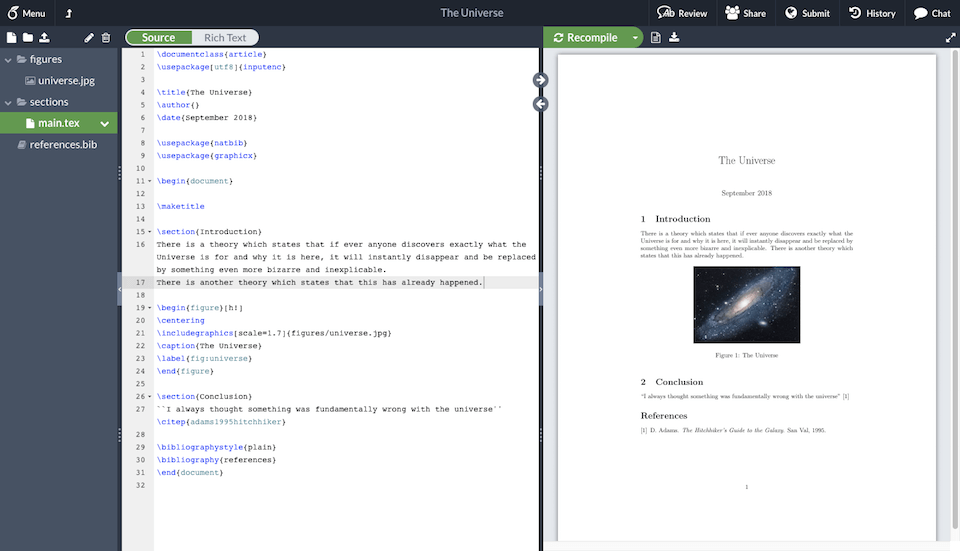
\includegraphics[width=0.7\linewidth]{overleaf.png}
	\caption{Layout of the Overleaf Online \LaTeX\ Editor.}
	\end{figure}
\end{frame}

\subsection{Documentation}

\begin{frame}[fragile]
	\frametitle{Documentation on your computer}
	If you've installed a full version of \TeX Live (as strongly recommended), the \LaTeX\ documentation about all you want to is in front of you. 
	\smallskip
	
	Open the command line and input the command \smallskip
	
	\mintinline{shell}|texdoc <docname>| \smallskip
	
	You can also use the online version \url{http://www.texdoc.net/}\\[0.5em]
	For example, you can use the following types for the \structure{docname}
	\begin{description}
		\item[tex] 		about \structure{\TeX}
		\item[article] 	about documentclass \structure{article}
		\item[beamer] 	about documentclass \structure{beamer} (used to create slides)
		\item[pgf]		about \structure{TikZ} and \structure{PGF} (used to draw graphs)
	\end{description}
	\smallskip
	Try to \alert{texdoc} about all new things and then you'll be an expert in \LaTeX.
\end{frame}

\section{Layout of the Document}
\begin{frame}
	\tableofcontents[currentsection,hideothersubsections]
\end{frame}

\subsection{A simple document}

\begin{frame}
	\frametitle{A simple document}
	A typical (simplest) \LaTeX\ example is presented here.
	\begin{example}
		\inputminted{latex}{examples/simple.tex}
	\end{example}
\end{frame}

\subsection{Basic document classes}

\begin{frame}[fragile]
	\frametitle{All begins with documentclass}
	\begin{definition}
		In a \LaTeX\ file, the \structure{first} line must be \\
		\mintinline{latex}|\documentclass[options]{class}|
	\end{definition}
	For example, you can use the following types for the \structure{class}
	\begin{description}
		\item[ariticle]	Write a report or an science article
		\item[report] 	Write a report
		\item[beamer]	Produce a lecture silde like this!
	\end{description}
	Some options can be added, for example, a typical case can be
	\mintinline{latex}|\documentclass[11pt,twoside,a4paper]{article}| \\[0.5em]
	Some details about the \structure{article} class will be introduced on the next page. More features about other classes and options can be found in the \LaTeX\ Document on your own.
\end{frame}

\begin{frame}[fragile]
	\frametitle{The article class}
	The \structure{article} class is the most basic class in \LaTeX, it provides you with some normalized structure and format for report writing. So usually you will use the following command as the first line of your tex document
	\mintinline{latex}|\documentclass[options]{article}| \\[0.5em]
	Some of the options values are listed below (the default values are \alert{alerted})
	\begin{itemize}
		\item \alert{10pt}, \structure{11pt}, \structure{12pt} or other sizes - the font size of the document
		\item \structure{a4paper}, \structure{a5paper}, \alert{letterpaper} - the size of paper
		\item \structure{fleqn} - make the math equations left aligned (default middle aligned)
		\item \structure{leqno} - display the serial numbers of math equations on the left (default on the right)
		\item \structure{titlepage}, \alert{notitlepage} - whether to make the title an entire page
		\item \alert{onecolumn}, \structure{twocolumn} - the number of columns of the document
		\item \structure{twoside}, \alert{oneside} - influence the position of something on the page
	\end{itemize}
\end{frame}

\begin{frame}
	\frametitle{Other classes}

	Read the source code of this project and you will learn much about the \structure{beamer} class. \\

	When writing a \alert{long} report, \structure{report} class can be used to provide some more layers of document and different type settings. It's very similar to the \structure{article} class, so it won't be specified. \\

	There are some other document classes such as \structure{book}, \structure{letter} and etc., but I think you will never use them.

\end{frame}

\subsection{Use packages}

\begin{frame}[fragile]
	\frametitle{Magic of packages}
	\LaTeX\ is a macro-based language, where most of useful commands are not built-in commands. These commands are defined in various packages, which should be included between \LC{\documentclass} and \LC{\begin{document}}.
	\begin{command}
		\mintinline{latex}|\usepackage[options]{package}|
	\end{command}
	There are some very useful packages that you may \alert{ALWAYS} include:
	\begin{description}
		\item[amsmath] Define various maths environments
		\item[amssymb] Define various maths symbols
		\item[geometry] Adjust the margin, paper size, and etc.
		\item[enumerate] Generate a list like this!
		\item[graphicx] Insert image of all types
	\end{description}
	The usages of these and more packages will be introduced further.
\end{frame}

\begin{frame}[fragile]
	\frametitle{Common packages}
	Here I provide a list of common used packages, you can start from using the commands of them after the lecture.

	\inputminted{latex}{examples/packages.tex}
\end{frame}

\subsection{Title page}
\begin{frame}[fragile]
	\frametitle{Title, Author and Date}
	It's very useful to generate a title on the first page of a document, in order to achieve it, these commands should first be added between \LC{\documentclass} and \mintinline{latex}{\begin{document}}.
	\begin{example}
		\begin{minted}{latex}
\title{title}
\author{author name}
\date{\today}
		\end{minted}
	\end{example}
	You can simply use \mintinline{latex}{\date{\today}} to display your system date now.\\[0.5em]
	Then in the \structure{document environment} (will be introduced in the next section), use the command \LC{\maketitle} to generate the title page.
\end{frame}

%\begin{frame}
%	\frametitle{Geometry package}
%	The settings of the layout of the pages is in \structure{geometry} package.
%	\begin{command}
%		\samplecommand{usepackage}\{geometry\}\\
%		\samplecommand{geometry}\{\structure{options}\}
%	\end{command}
%	Some of the \structure{options} are listed below:
%	\begin{itemize}
%		\item \structure{paper} - same as the paper settings in documentclass
%		\item \structure{layout} - use another type of paper's layout
%		\item \structure{left/right} - the blank length on the left/right
%		\item \structure{top/bottom} - the blank length on the top/bottom
%	\end{itemize}
%	\begin{example}
%		\samplecommand{geometry}\{paper=a4paper,layout=a5paper\}
%		\samplecommand{geometry}\{left=2.5cm,right=2.5cm,top=2.5cm,bottom=2.5cm\}
%	\end{example}
%\end{frame}

\section{Document Body}

\begin{frame}
	\tableofcontents[currentsection,hideothersubsections]
\end{frame}

\subsection{Body}
\begin{frame}[fragile]
	\frametitle{Main body of document}
	The main body of your document which starts with \mintinline{latex}{\begin{document}} and ends with \mintinline{latex}{\end{document}} is called the \structure{document} environment. All of the contents you'd like to display should be in it, and it \alert{MUST} be \alert{unique} in the whole file.
	\begin{example}
		\begin{minted}{latex}
\begin{document}
    \maketitle
    \newpage   %start the following contents in a new page
    \tableofcontents %automatically generate a table of content
    \newpage
    Hello, \LaTeX !
    % TODO: Add more contents
    ...
\end{document}
		\end{minted}
	\end{example}
	The position and order of title page and table of contents can be arbitrary, and there can be multiple table of contents in one document.
\end{frame}

\subsection{Layers}

\begin{frame}[fragile]
	\frametitle{Dividing into sections}
	\begin{command}
		\begin{multicols}{2}
			\begin{minted}{latex}
\section{name}
\subsection{name}
\subsubsection{name}
			\end{minted}
			\begin{minted}{latex}
\section*{name}
\subsection*{name}
\subsubsection*{name}
			\end{minted}
		\end{multicols}
		\vspace{-0.5em}
	\end{command}
	The default style of sections is like\\
	\structure{1 Example Section Name}\\
	\structure{1.1 Example Subsection Name}\\
	\structure{1.1.1 Example Subsubsection Name}\\[0.5em]
	If a star(\alert{*}) is added, the sequence number will be hidden, and it won't be added to the table of contents.\\
	\alert{Note:} (Sub)sections can be sorted into commands, not environments, so it doesn't have \LC{\begin} and \LC{\end} clauses. However, the whole contents between two (sub)sections is belonged to the former (sub)section.
\end{frame}

\begin{frame}[fragile]
	\frametitle{Other structures - Chapter, Part and Paragraph}
	\begin{command}
		\begin{multicols}{2}
			\begin{minted}{latex}
\chapter{name}
\part{name}
\paragraph{name}
\subparagraph{name}
			\end{minted}
			\begin{minted}{latex}
\chapter*{name}
\part*{name}
\paragraph*{name}
\subparagraph*{name}
			\end{minted}
		\end{multicols}
		\vspace{-0.5em}
	\end{command}
	In document classes such as \structure{report} and \structure{book}, some outer structures of \structure{section} (\LC{\chapter} and \LC{\part}) can be used. \\[0.5em]
	\LC{\paragraph} and \LC{\subparagraph} are used for the title of small paragraphs in a (sub)section.\\[0.5em]
	If a star(\alert{*}) is added, the effect will be the same as in the sections (sequence numbers will be hidden).
\end{frame}

\section{Learn more - syntax of \LaTeX}

\begin{frame}
	\tableofcontents[currentsection,hideothersubsections]
\end{frame}

\subsection{Command}

\begin{frame}[fragile]
	\frametitle{The common syntax of \LaTeX\ commands}
	All \LaTeX\ commands have the following syntax \\

	\mintinline{latex}{\commandName<specialArgs>[optionalArgs]{requiredArgs}}
	\begin{description}
		\item[specialArgs]	Seldom used in basic usage, for certain special usages in some packages
		\item[optionalArgs]	Used to define mode of the command, if not specified, \LaTeX\ will use the default mode
		\item[requiredArgs]	Must be filled
	\end{description}
	If you want to connect a letter after a command, a space must be appended after the command or \LaTeX\ won't be able to compile it correctly. But two commands can be directly connected since there is a \mintinline{latex}{\} before each command.
\end{frame}

\subsection{Environment}

\begin{frame}[fragile]
	\frametitle{The common syntax of \LaTeX\ environments}
	All \LaTeX\ environments have the following syntax \\

	\begin{minted}{latex}
\begin{environmentName}<specialArgs>[optionalArgs]{requiredArgs}
    % ...
\end{environmentName}
	\end{minted}
	\structure{specialArgs}, \structure{optionalArgs}, \structure{requiredArgs} are similar to those in a \structure{command} \\

	It is recommended to have a tab indent in each environment or your tex codes will be difficult to read by others or even \alert{yourself}.
\end{frame}
